% !TEX encoding   = UTF8
% !TEX spellcheck = ru_RU

\section{Теоретическое описание}
%%==============================================================
\begin{frame}{Метод Галёркина (DG)}
	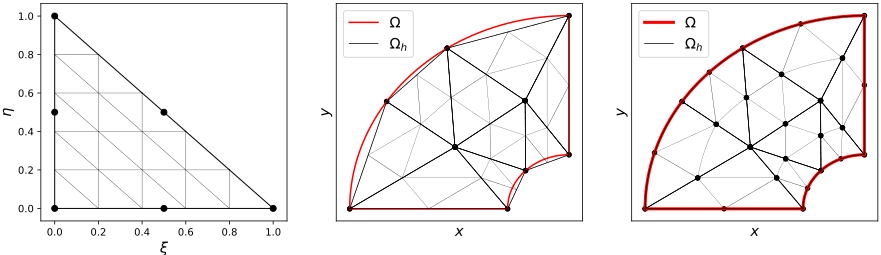
\includegraphics[width=1\textwidth]{standart_quad_lin_example}
	\begin{block}{Основная идея метода:}
		\begin{itemize}
			\item Пространство \(\Omega\) разбивается на элементы  \(K_{ie}\)
			\item Решение ищется в виде: \(\mathbf U(\mathbf x, t)\biggm|_{\mathbf{x} \in K_{ie}} = \sum\limits_{m=1}^{K_f} \mathbf u_m(t)\, \varphi_m(\mathbf x)\)
			\item Система уравнений: \[\frac{\mathrm d\mathbf u_m}{\mathrm d t} = \mathbf R_m = -\oint_{\Sigma_{ie}} \ldots\: \mathrm d\Sigma\quad +\quad \int_{K_{ie}} \mathbf \ldots\: \mathrm d\mathbf x\]
		\end{itemize}
	\alert{Необходимо вычислить поверхностные и объемные интегралов}
	\end{block}
\end{frame}

\note{
	Начну с краткого описания метода Галёркина с разрывными базисными функциями. Основная идея заключается в следующем: область \(\Omega\), в которой ищется решение, разбивается на множество непересекающихся элементов, образующих расчётную сетку. Ячейки сетки стыкуются друг с другом по граням, как это показано на рисунке сверху. Решение в каждой ячейке сетки представляется в виде линейной комбинации базисных функций. Такой вид решения подставляется в исходную систему уравнений, а дальше производится интегрирование по \todo{каждой} ячейке расчётной области. В случае, когда базисные функции ортонормированы, можно упростить систему. Не вдаваясь в подробности вывода, на слайде показан общий вид этой системы. Система содержит невязку, которая представляет из себя сумму поверхностного и объемного интегралов. Базисными функциями в солвере ZOOM являются полиномы некоторой степени. Поэтому подынтегральные выражения в невязке "--- это полиномы некоторой степени. Для решения системы уравнений, необходимы методы вычисления объемных и поверхностных интегралов в невязке.
}


%%==============================================================
\begin{frame}{Интегрирование по элементам}
	\begin{columns}
		\begin{column}{0.75\textwidth}
			Стандартный элемент \(\hat \Omega\) отображается в физическое пространство:
			\[
			\left\{\begin{array}{l}
			x = x (\xi, \eta, \zeta), \\
			y = y (\xi, \eta, \zeta), \\
			z = z (\xi, \eta, \zeta), \\
			\end{array}\right.\quad \xi, \eta, \zeta \in \hat \Omega
			\]
			Для интегрирования по \(\hat \Omega\) используют некоторые кубатурные правила:
			\[
			\iiint\limits_{\hat\Omega}F(\xi, \eta, \zeta) \:\mathrm d \hat\Omega = \sum_{i = 0}^{N} F(\xi_i, \eta_i, \zeta_i) \alpha_i
			\]
		\end{column}
		\begin{column}{0.25\textwidth} \\
			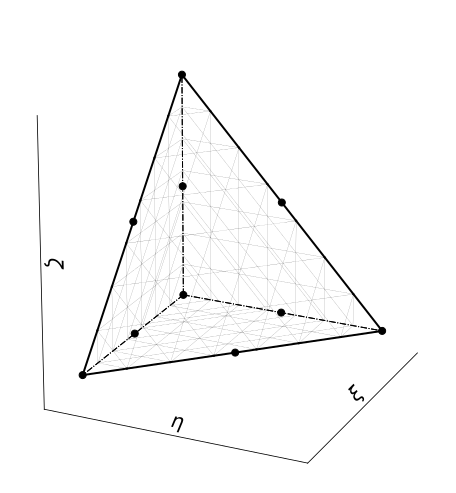
\includegraphics[width=1\textwidth]{standart_tetra.png}
			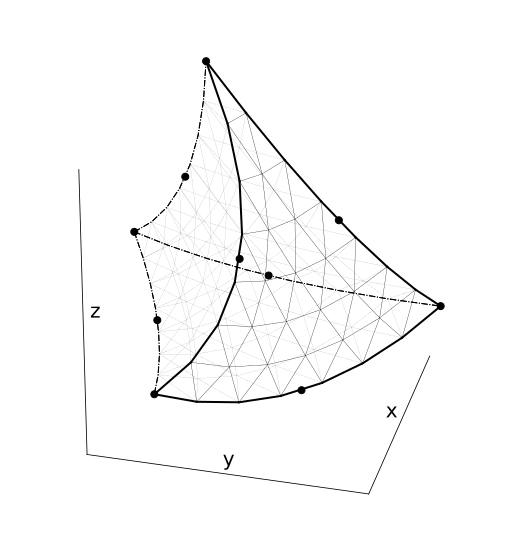
\includegraphics[width=1\textwidth]{transformed_tetra.png}
		\end{column}
\end{columns}
	Интегрирование по \(K_{ie}\) сводится к интегрированию по \(\hat \Omega\):
	\[
	\newcommand*{\vecxi}{\xi, \eta, \zeta}
	\iiint\limits_{K_{ie}}F(x, y, z)\: \mathrm d\mathbf x =\\
	\iiint\limits_{\hat\Omega}F\big(x(\vecxi), y(\vecxi), z(\vecxi)\big) \left|\det\mathbf J(\vecxi)\right|\:\mathrm d\xi\,\mathrm d\eta\, \mathrm d\zeta
	\]
\end{frame}

\note{
	Теперь рассмотрим способ интегрирования по элементам расчётной области. Элементы, на которые разбивается область, вообще говоря, могут быть произвольными. Однако вычисление интегралов по произвольным ячейкам "--- практически невыполнимая задача. Поэтому вводятся стандартные элементы, для которых известны методы получения точных значений интегралов от полиномов заданной степени, или, проще говоря, кубатурные правила. Эти элементы, в свою очередь, отображаются в физическое пространство, используя преобразования координат. Теперь интегрирование по элементам расчётной области можно свести к интегрированию по стандартному элементу, используя нижеприведённую формулу.
}


%%==============================================================
\begin{frame}{Преобразования элементов}
	\begin{columns}
		\begin{column}{0.45\textwidth}
			\begin{block}{Вид преобразования:\\}
				\[
				\left\{\begin{array}{l}
				x = \sum_{i=1}^n x_i N_i(\xi, \eta, \zeta), \\
				y = \sum_{i=1}^n y_i N_i(\xi, \eta, \zeta), \\
				z = \sum_{i=1}^n z_i N_i(\xi, \eta, \zeta), \\
				\end{array}\right.
				\]
				\(\xi, \eta, \zeta \in \hat \Omega\), \\
				\((x_i, y_i, z_i)\) {\small "--- координаты \(i\)-го узла в физическом пространстве,} \\ 
				\(N_i\) {\small "--- функция формы, равная единице в \(i\)-ом узле и нулю в других узлах стандартного элемента}
			\end{block}
		\end{column}
		\begin{column}{0.55\textwidth}
			\begin{block}{Стандартные элементы:}
				\begin{columns}[t]
					\begin{column}{0.5\textwidth}
						\small
						\centering
						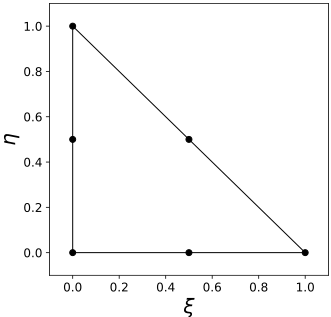
\includegraphics[width=1\textwidth]{tri_standart}
						\medskip
						Двумерный симплекс
						\includegraphics[width=1\textwidth]{rect_standart}
						Квадрат
					\end{column}
					\begin{column}{0.5\textwidth}
						\small
						\centering
						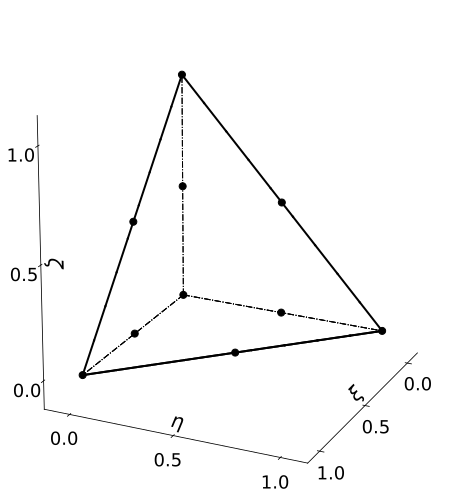
\includegraphics[width=1\textwidth]{tetra_standart}
						\medskip
						Трёхмерный симплекс
						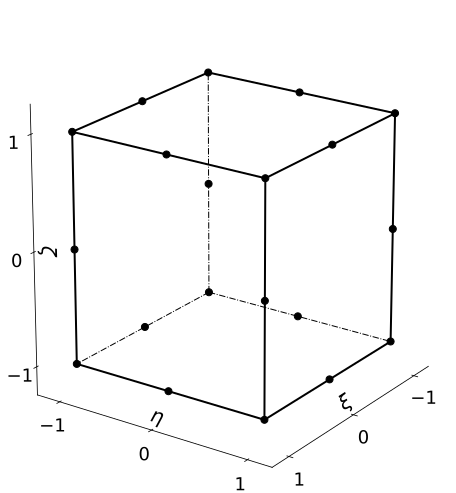
\includegraphics[width=0.9\textwidth]{hexa_standart}
						Куб
					\end{column}
				\end{columns}
			\end{block}
		\end{column}
	\end{columns}
\end{frame}

\note{
	В качестве стандартных элементов используются симметричные фигуры, такие, как куб, квадрат, трёхмерный и двумерный симплексы. В работе используются преобразования, которые могут быть представлены в виде суммы произведения функций форм на координаты узлов в физическом пространстве, как это показано на слайде. Количество узловых точек на рёбрах определяет тип элемента. В программе их два: <<линейный>> или <<квадратичный>>. Так, в случае <<линейных>> элементов, количество узлов на каждом ребре ячейки равно двум. Для аппроксимации сложной геометрии небольшим количеством элементов простых <<линейных>> многогранников уже не достаточно. Возникает необходимость вводить <<квадратичные>> элементы, каждое ребро которых представлено тремя узловыми точками. На слайде справа показаны стандартные элементы с выделенными узловыми точками.
}


%%==============================================================
\begin{frame}{Кубатурные правила}
	\bigskip
	\begin{columns}
		\begin{column}{0.3\textwidth}
			\centering
			\includegraphics[width=1\textwidth]{6_rect_to_tri}
			\small
			Исходный квадрат
		\end{column}
		\begin{column}{0.3\textwidth}
			\centering
			\includegraphics[width=1\textwidth]{6_tri_not_opti}
			\small
			Гауссовы кубатуры, \(N = 16\)
		\end{column}
		\begin{column}{0.3\textwidth}
			\centering
			\includegraphics[width=1\textwidth]{6_tri_opti}
			\small
			Оптимальные кубатуры, \(N = 12\)
		\end{column}
	\end{columns}
	\medskip
	\begin{block}{В программе используются 2 типа кубатур:}
		\begin{itemize}
			\item Декартово произведение одномерных квадратур Гаусса
			\begin{itemize}
				\item Произвольный порядок
				\item Хорошо подходят для гексаэдров
			\end{itemize}
			\item Оптимизированные кубатурные правила
			\begin{itemize}
				\item Сложность получения для высоких порядков
				\item Хорошо подходят для тетраэдров
			\end{itemize}
		\end{itemize}
	\end{block}
\end{frame}

\note{
	Для достижения поставленной задачи, помимо преобразований элементов, необходимо также рассмотреть правила интегрирования. В программе испольуются 2 типа кубатур: гауссовы кубатуры и оптимизированные кубатуры. В случае шестигранников и квадратов, квадратурные правила могут быть получены из одномерных квадратур Гаусса как их декартово произведение. Пример гауссовых кубатур, полученных таким образом для квадрата, приведен на левом русунке. Преобразования гексаэдров обладают определенными свойствами, которые позволяют снизить количество точек в квадратурных правилах, построенных как декартово произведение одномерных правил. У тетраэдров напрямую использовать квадратурные правила нельзя. Однако можно, впрочем, получить кубатурные правила для тетраэдра из кубатурных правил для гексаэдров, используя преобразование, как это показано на слайде: из исходного квадрата получен треугольник. Однако таким образом полученные правила интегрирования обладают недостатками: нессиметричность, сгущение в одной точке, неоптимальное количество кубатурных точек. На 2-м и 3-м рисунках сверху приведено сравнение оптимальных и гауссовых кубатурных правил 6 порядка для треугольника. Видно, что количество точек у оптимальной кубатуры меньше. Для тетраэдров в программе пока что были использованы оптимизированные симметричные кубатурные правила.
}


\section{Программная реализация}
%%==============================================================
\begin{frame}{Элементы реализации в коде ZOOM DG}
	\bigskip
	\begin{columns}
		\begin{column}{0.5\textwidth}
			\centering
			\begin{adjustbox}{max totalsize={1.1\textwidth}{!},center}
				\begin{tikzpicture}[nodes={font=\ttfamily\tiny, draw},
					rounded corners, level distance=5ex, >=Stealth]
					\graph [layered layout, components go right top aligned, edge=<-]
					{
						QRCell -> QRHexa -> {
							QRHexaOptimized,
							QRHexaGaLe
						};
						QRCell ->[blue] QRTetra[blue, text=blue]
						->[blue] QRTetraOptimized[blue, text=blue]
						->[blue] {
							QRTetraFirst[blue, as={QRTetra\_1\_1}],
							QRTetraJth[blue, as={...}],
							QRTetraNth[blue, as={QRTetra\_8\_43}]
						};
						QRTetra ->[blue, dashed] QRTetraGaLe[blue, dashed, text=blue, edge=dashed];
					};
					
					\begin{scope}[on background layer]
					\node [draw, rounded corners,
					fit=(QRCell) (QRHexaOptimized) (QRTetraGaLe) (QRTetraNth)] {};
					\end{scope}
				\end{tikzpicture}
			\end{adjustbox}
			\small
			Правила интегрирования
		\end{column}
		\begin{column}{0.5\textwidth}
			\centering
			\begin{adjustbox}{max totalsize={1.1\textwidth}{!},center}
				\begin{tikzpicture}[nodes={font=\ttfamily\tiny, draw},
					rounded corners, level distance=10ex, >=Stealth]
					\graph [layered layout, components go right top aligned, edge=<-]
					{
						ShapeFunctionSet3D -> {
							HexaLinearElement[as=\tcol{HexaLinear\\Element}],
							HexaQuadraticElement[as=\tcol{HexaQuadratic\\Element}]
						};
						ShapeFunctionSet3D ->[blue] {
							TetraLinearElement[blue, as=\tcol{TetraLinear\\Element}],
							TetraQuadraticElement[blue, as=\tcol{TetraQuadratic\\Element}]
						};
					};
					\begin{scope}[on background layer]
					\node [draw, rounded corners,
					fit=(ShapeFunctionSet3D) (HexaLinearElement) (TetraQuadraticElement)] {};
					\end{scope}
				\end{tikzpicture}
			\end{adjustbox}
			\small
			Преобразования элементов
		\end{column}
	\end{columns}
	\bigskip
	\begin{block}{Вспомогательные скрипты:}
		\begin{itemize}
			\item Скрипт на \code{Python} для генерации кода симметричных правил интегрирования
			\item Скрипт с использованием библиотеки символьной математики \code{SymPy} для генерации кода функций преобразования тетраэдров
		\end{itemize}
	\end{block}
	\alert{Проведено сравнение с аналитическими решениями}
\end{frame}

\note{
	После изучения математического аппарата, я зан\'ялся написанием кода.	Структура кода расчётного модуля ZOOM DG выстроена таким образом, что для внедрения поддержки тетраэдральных элементов достаточно добавить правила преобразования и правила интегрирования. Идеи в коде представлены в виде типов. На рисунках на слайде показаны классовые иерархии кубатурных правил и правил преобразования. Синим выделены фрагменты, добавленные для поддержки тетраэдральных элементов. Код для правил интегрирования и для преобразований элементов состоит из множества функций, в которых легко допустить ошибку. Чтобы автоматизировать процесс и избавить себя от рутины, на \code{Python} с использованием библиотеки символьной математики \code{SymPy}, были написаны скрипты для генерации кода. Для проверки на наличие ошибок при интегрировании, были проведены сравнения с аналитическими решениями.
}


%%==============================================================
\section{Тестирование}
\begin{frame}{Обтекание цилиндра сжимаемым невязким потоком}
	\begin{center}
		\includegraphics[width=0.8\textwidth]{cylinder_tetra_fine_K3_Mach}
	\end{center}
	\begin{columns}[t]
	\begin{column}{0.55\textwidth}
		\begin{block}{Характеристики расчётной области:}
			\begin{itemize}
				\item высота цилиндра --- 100 м
				\item радиус цилиндра --- 1 м
				\item радиус расчётной области --- 1000 м
			\end{itemize}
		\end{block}
	\end{column}
	\begin{column}{0.45\textwidth}
		\begin{block}{Начальное поле:}
			\begin{itemize}
				\item давление \(p_\infty = 100\,000\) Па
				\item плотность \(\rho_\infty = 1.19\) кг/\(\text{м}^3\)
				\item скорость потока  \(u_\infty = 50\) м/с
			\end{itemize}
		\end{block}
	\end{column}
	\end{columns}
\end{frame}

\note{
	После внедрения кода, необходимо было провести тестовые расчёты. В качестве тестовой задачи рассматривается обтекание цилиндра невязким сжимаемым дозвуковым потоком. Характерная картина течения изображена на слайде. Обтекание цилиндра выбрано по следующим причинам: задача простая, а решение задачи экспериментально и теоретически изучено. Обтекаемое тело имеет криволинейную форму, что позволяет протестировать разные типы преобразования координат и выяснить, как они влияют на ошибку в решении. Для выполнения расчёта необходимо построить расчётную сетку, а также задать начальные и граничные условия. Характеристики расчётной области, а также начальное поле описаны на слайде.
}


%%==============================================================
\begin{frame}{Подготовка расчётной сетки}
	\bigskip
	\begin{columns}
		\begin{column}{0.45\textwidth}
			\textbf{\huge Gmsh}
			\begin{block}{Параметры скрипта для тетраэдральной сетки:}
				\begin{enumerate}
					\item Внешний радиус
					\item Радиус цилиндра
					\item Кол-во ячеек вдоль радиуса
					\item Размеры ячеек
					\begin{itemize}
						\item коэффициент прогрессии
					\end{itemize}
				\end{enumerate}
			\end{block}
		\end{column}
		\begin{column}{0.55\textwidth}
			\centering
			\includegraphics[width=1\textwidth]{tetra_mesh_full}\\[3ex]
			\includegraphics[width=1\textwidth]{tetra_mesh}
		\end{column}
	\end{columns}
\end{frame}

\note{
	Расчётная сетка была построена с использованием трёхмерного генератора конечно-элементных сеток \code{Gmsh}. Сперва для знакомства с программой был написан скрипт для генерации гексаэдральных расчётных сеток, а затем скрипт для построения сеток из тетраэдральных элементов. Так как задача стационарная, а решение симметрично в верхней и нижней полуплоскостях, то сетка строилась только для половины расчётной области цилиндра. На слайде сверху изображена вся расчётная область, а снизу часть вокруг самого цилиндра. Расчёты проводились с различными степен\'ями базисных полиномов для двух видов сеток: с <<линейными>> и <<квадратичными>> элементами.
}


%%==============================================================
\begin{frame}{Оценка ошибки сопротивления}
	\medskip
	\centering
	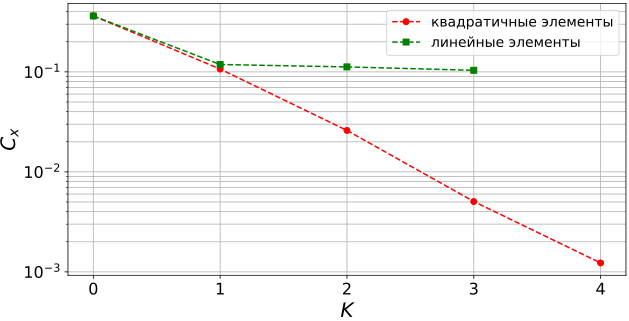
\includegraphics[width=1\textwidth]{Cx}
	Убывание ошибки в определении коэффициента сопротивления~\(C_x\) в зависимости от порядка базисных функций~\(K\)
\end{frame}

\note{
	В следствие парадокса Д'Аламбера, сопротивление цилиндра в точном решении должно быть равным нулю. Поэтому по коэффициенту сопротивления можно оценить ошибку в решении. На слайде показано убывание ошибки сопротивления в зависимости от порядка базисных функций. Видно, что для \(K = 0\) и \(K = 1\) ошибки у <<квадратичных>> и <<линейных>> тетраэдров идентичны. Но с дальнейшим увеличением \(K\) ошибка в случае <<линейных>> элементов практически не убывает, в отличние от <<квадратичных>> элементов. Причем с увеличением степени базисных функций на единицу, ошибка убывает примерно на порядок. 
}


%%==============================================================
\begin{frame}{Оценка полного давления за цилиндром}
	\begin{columns}
		\begin{column}{0.4\textwidth}
			\begin{block}{Полное давление:}
				\[p_{0\infty} = p_\infty \left(1 + \frac{\gamma-1}{2}M_{\infty}^2\right)^\frac{\gamma}{\gamma - 1}\]
				\(p_{0\infty}\)~должно сохраняться во всём поле течения. За цилиндром видно падение давления. Можно оценить ошибку в этой точке:
				\(\Delta p_0 = p_{0\infty} - p_0(\mathbf x_b)\)
			\end{block}
		\end{column}
		\begin{column}{0.6\textwidth}
			\bigskip
			\centering
			\includegraphics[width=1\textwidth]{K2_quad}
			\small
			Поле полного давления при~\(K = 2\)
		\end{column}
	\end{columns}
\end{frame}

\note{
	Рассмотрим поле полного давления.	Задача стационарная, жидкость невязкая, следовательно полное давление должно сохранятся во всём поле течения. Видно, что непосредственно за цилиндром есть область падения полного давления. Обозначим эту точку за \(\mathbf x_b\). И по величине \(\Delta p_0\) попытаемся определить ошибку в решении. Хочу отметить, что нечеткость картины течения на слайде связана с грубой визуализацией поля. На самом деле картина даже на такой грубой сетке довольно гладкая.
}


%%==============================================================
\begin{frame}{Оценка полного давления за цилиндром}
	\medskip
	\centering
	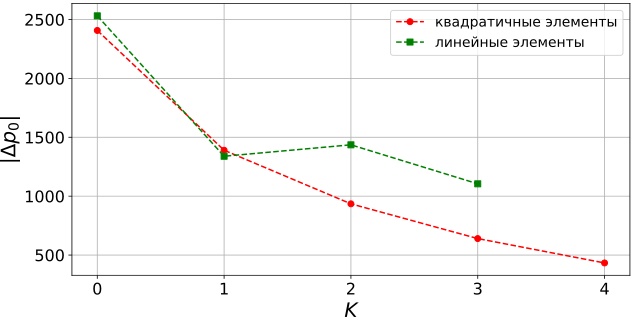
\includegraphics[width=1\textwidth]{p0}
	Убывание ошибки в определении полного давления~\(p_0\) в зависимости от порядка базисных функций~\(K\)
\end{frame}

\note{
	На слайде показано убывание ошибки в зависимости от степени базисных функций в точке~\(\mathbf x_b\). Картина аналогична тому, что мы видели при оценке ошибки сопротивления: при \(K = 0\) и \(K = 1\) ошибки идентичны, а при увеличении порядка~\(K\) ошибка в случае <<квадратичных>> элементов уменьшается больше, чем в случае <<линейных>>.
}